%% This is an example first chapter.  You should put chapter/appendix that you
%% write into a separate file, and add a line \include{yourfilename} to
%% main.tex, where `yourfilename.tex' is the name of the chapter/appendix file.
%% You can process specific files by typing their names in at the 
%% \files=
%% prompt when you run the file main.tex through LaTeX.
\chapter{Experiments}
\label{chap:experiments}

% % remove all spaces between columns in tables
% \setlength{\tabcolsep}{0.3pt}
% % remove all spaces below captions
% \setlength{\belowcaptionskip}{-5pt}

In this chapter, we first introduce our synthetic dataset, this dataset contains IMU measurements and corresponding visual frames, it also provides the ground truth IMU-camera pose to be used in evaluation stage. We then perform some experiments to show that our visual-inertial odometry has good accuracy and low computational cost in several different experimental settings.

\section{Synthetic Dataset}
\label{sec:sync_data}

\begin{table}[t]
\centering
\begin{tabular}{|c || P{2.5cm} | P{2.5cm} | P{6.5cm}|} 
\hline
 Name & Overall Duration $\left[ s \right]$ & Travelled Distance $\left[ m \right]$ & Description \\
 \hline
 001 & 30.0 & 165.97 & Pure movement without rotation \\ 
 002 & 30.0 & 0.0 & Pure rotation without translation \\ 
 003 & 30.0 & 118.99 & Random straight trajectory \\ 
 004 & 120.0 & 257.71 & Random circle-like trajectory \\ 
 \hline
\end{tabular}
     \caption{Trajectories we create for experiments, the datasets are named after the corresponding trajectories. Noted that \textbf{001} and \textbf{002} are ideal trajectories to test the correctness and performance of ESKF IMU integration. The trajectory \textbf{003} and \textbf{004} try to simulate the trajectories of micro helicopter by setting the similar velocity and pose.}
    \label{table:tb1}
\end{table}

%\begin{figure}
%\centering
%	\begin{subfloat}[Trajectory 003]{
%		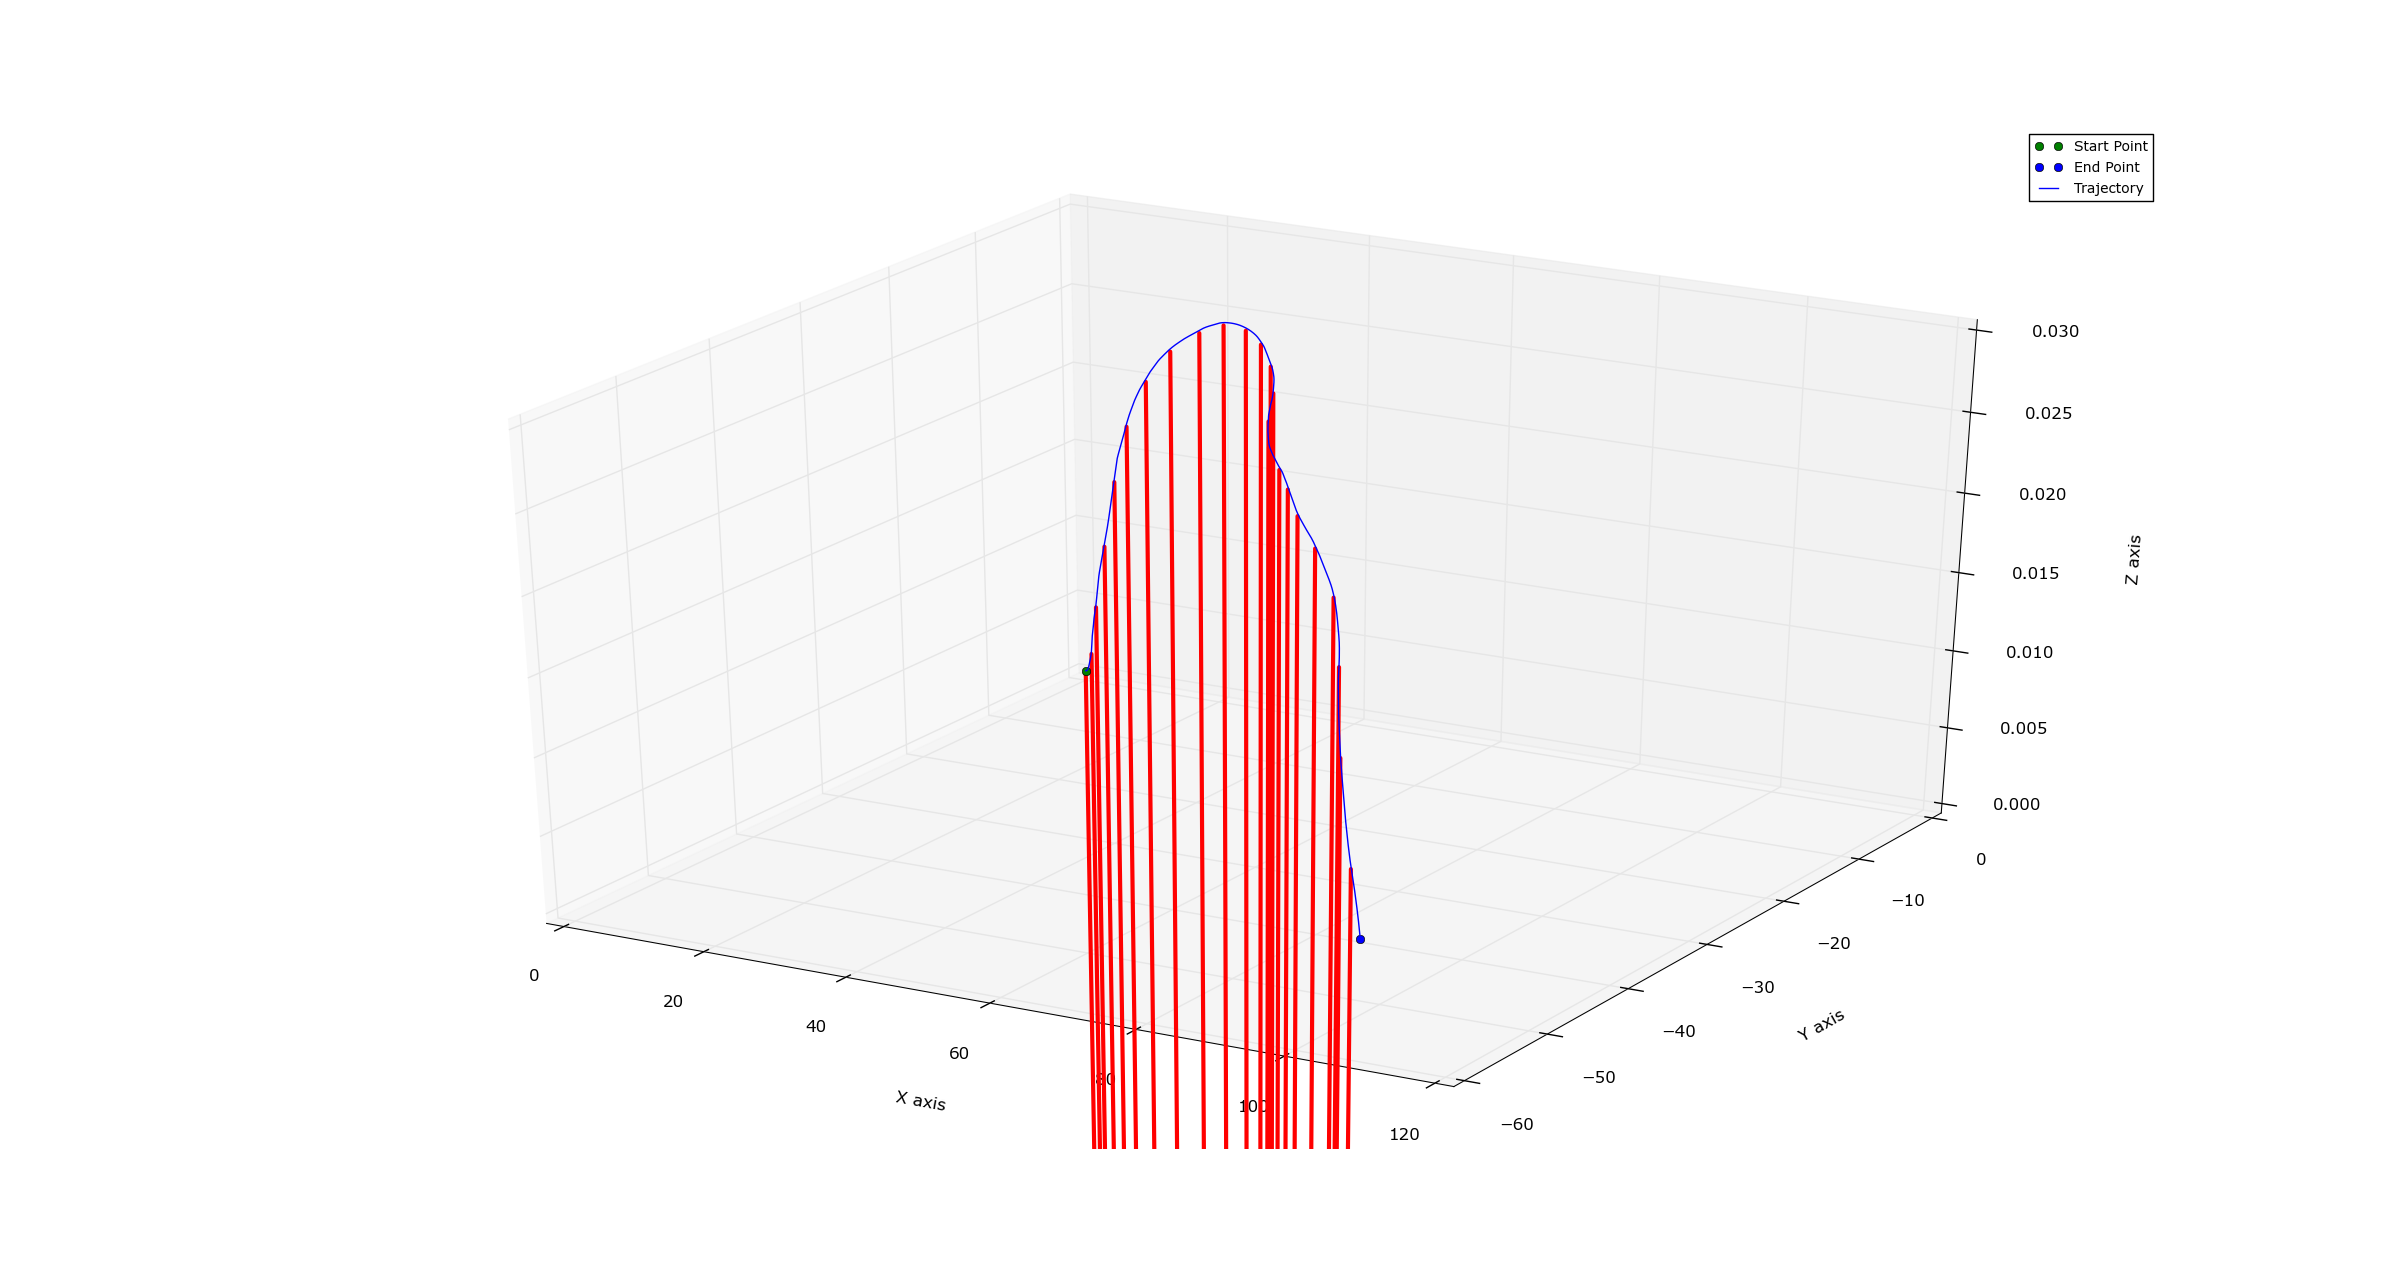
\includegraphics[width=0.4\textwidth]{CONTENT/Figure/Figure5-1a.png}
%		\label{fig:fig5-1-a}}
%	\end{subfloat}\qquad
%	\begin{subfloat}[Trajectory 004]{
%		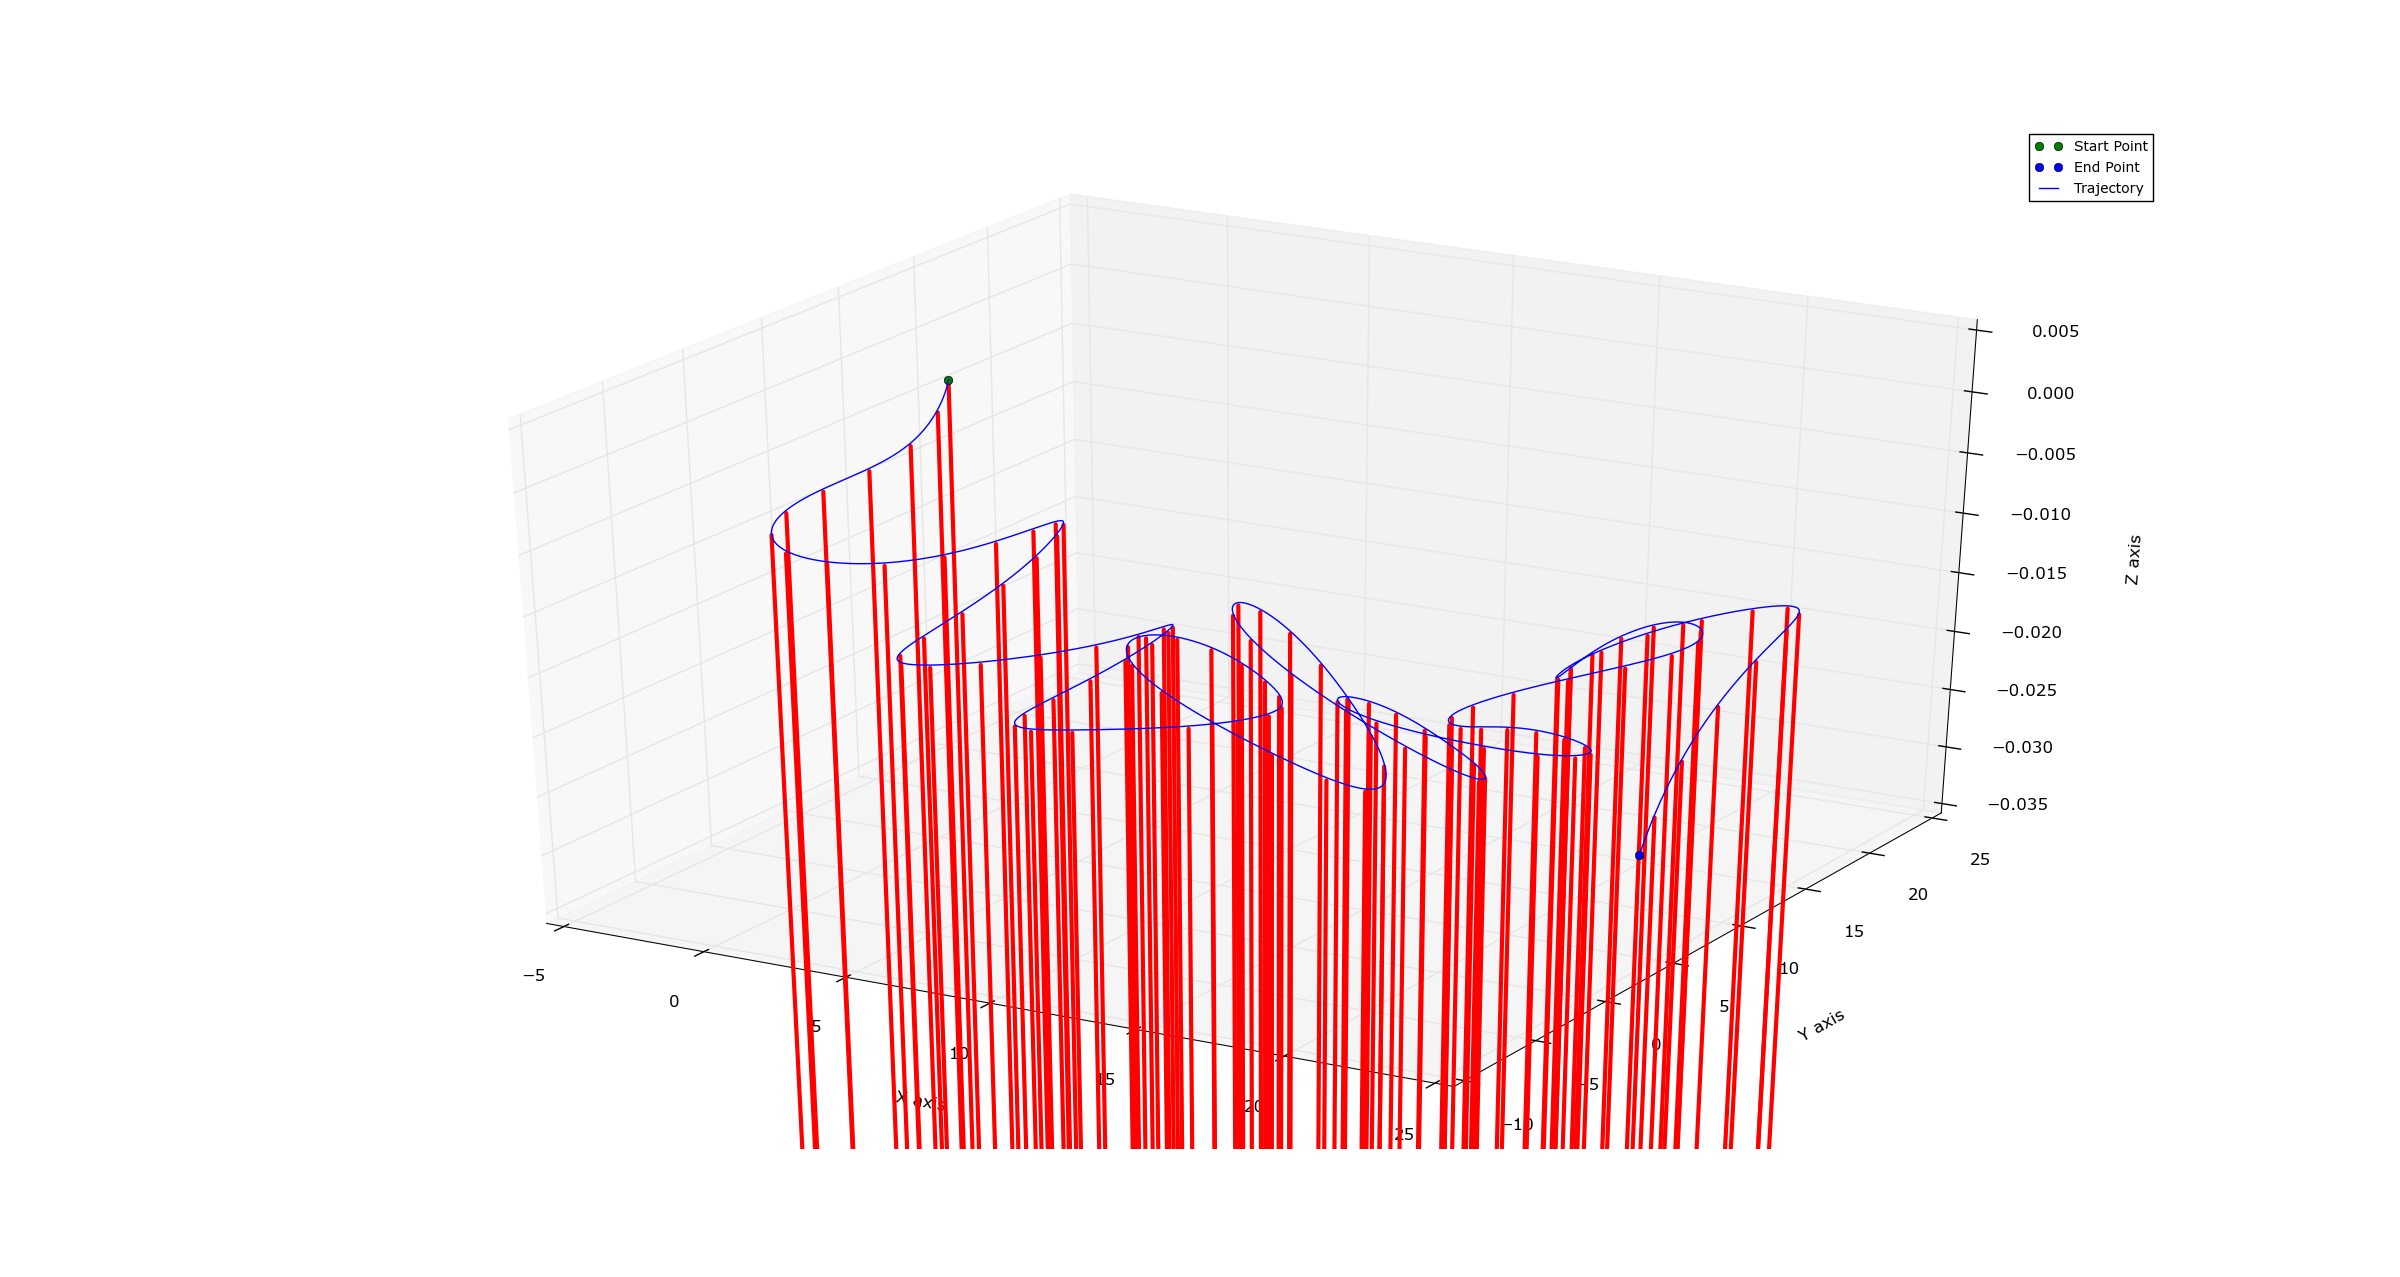
\includegraphics[width=0.4\textwidth]{CONTENT/Figure/Figure5-1b.png}
%		\label{fig:fig5-1-b}}
%	\end{subfloat}
	
	%\hspace*{\fill} % separation between the subfigures
	
%	\caption{Visualization of trajectory \textbf{003} and trajectory \textbf{004}. } 
%	\label{fig:fig5-1}
%\end{figure}

We use a synthetic IMU-camera dataset in this master thesis because it has following advantages rather than real dataset
\begin{itemize}
\item {Noises in synthetic dataset is controllable. Though we have considered the noise model in our work, the types of noises in real data varies. Besides, denoising from such as IMU sensor is beyond the content of this master thesis. }
\item {Synchronization between IMU and camera is annoying. Though we know the frequency of camera and IMU from datasheet or introduction, the real output might still differ, \eg, the first image frame might correspond to fourth IMU measurement in first trial but changes to fifth IMU measurement in next trial. In synthetic data, we could use aligned IMU and camera data.}
\item {Synthetic data is more flexible. We could generate the special trajectory, \ie, a pure rotation sequence. However it is hard to create such a sequence in real platform.}
\item {Synthetic data can provide accurate ground truth data at each timestamp. In real platform, a evaluation of position drift usually only happens at end point, \eg, setting the start point as same as end point and measure the drift. Motion capture system can provide ground truth data at each timestamp, however accuracy of such system usually is not high as synthetic data.}
\item {Numerous calibration steps are saved. In real equipment, it is normal to calibrate the device again after several uses. We can ignore the calibration process in simulated platforms.}
\end{itemize}
Also to best of our knowledge, there is no open sourced IMU-camera synthetic data set, hence we decide to generate our own IMU-camera synthetic dataset.

\

\textbf{Trajectory} We start to generate synthetic data by first defining the trajectory of our IMU-camera platform. As we explain before, we assume the camera and IMU sensor share an identical pose in all our experiments for simplification. We have created four different types of trajectory showed in Table \ref{table:tb1}. Dataset \textbf{001} and Dataset \textbf{002} is used to evaluate the performance of ESKF IMU integration as we use ground-truth data in \textit{correction step}; And Dataset \textbf{003} and Dataset \textbf{004} test the performance of visual-inertial odometry which \textbf{004} has longer travelled distance. We have made following several general assumptions of trajectories,
\begin{itemize}
\item{We assume the initial position of trajectory as $(0, 0, 0)$ in global frame, and initial orientation as quaternion $(1, 0, 0, 0)$ which points at the positive z axis of global coordinate system.}
\item{We assume the second derivative of position and orientation remains constant within two successive sensor samplings.}
\item{We assume the second derivative of position and orientation obeys a normal distribution with additional white Gaussian noise.}
\end{itemize}

\

\textbf{Synthetic IMU data} We then use IMUSim \cite{young2011imusim} to simulate IMU data by our customized trajectory. IMUSim is a powerful python-based open-sourced IMU simulation tool, which models a wide range of real-world environments and/or external noises. To obtain more realistic IMU data, we set the output frequency of IMU as 100 [Hz], sensitivity of gyroscope is 1200 [deg/s] and sensitivity of accelerometer is 4 gravity. The whole IMU model is noise-free with some additional white Gaussian noise. Overall we have 3-vector gyroscope readings, 3-vector accelerometer readings, 3-vector ground truth position, 4-vector ground truth orientation from IMUSim for single IMU sampling.

\

\textbf{Synthetic visual data} Blender \cite{wiki:blender} is the main tool that creates virtual scene for our experiments. We use high-frequency grass-like texture and sun light to simulate the outdoor environment. Thanks to Python interface of Blender, we can import our defined trajectory, and then render a video clip as our visual data set. Here we use linear interpolation for position, \eg, a position $\vec{p}$ between two successive ground truth positions $\vec{p}_t$ and $\vec{p}_{t+1}$ can be computed as
\begin{align}
	\label{e1}
	\Delta{t} &= \frac{t_p - t}{t_1 - t} \\
	\vec{p} &= \vec{p}_t + (\vec{p}_{t+1} - \vec{p}_{t})\Delta{t}
\end{align}
where $t_p$, $t_1$ and $t$ is time when $\vec{p}$, $\vec{p}_t$ and $\vec{p}_{t+1}$ has been measured. We use \textit{Slerp} to interpolate between two quaternion $\vec{q}_t$ and $\vec{q}_{t+1}$ using Equation (\ref{e1}), we obtain the result $\vec{q}$ as
\begin{align}
	\vec{q} &= \frac{\vec{q}_{t}\sin{((1-\Delta{t})\theta)}+\vec{q}_{t+1}\sin{(\Delta{t}\theta})}{\sin{\theta}}
\end{align}
where $\theta$ is the half angle between quaternion $\vec{q}_t$ and $\vec{q}_{t+1}$. The resolution of image is $752 \times 480$, and intrinsic matrix of our virtual pin-hole camera is pre-defined, which is showed in Table \ref{table:tb2}. The output frequency is set to 25 [Hz], three times less than IMU output frequency.

\begin{table}[t]
\centering
\begin{tabular}{|c || P{1cm} | P{1cm} | P{1cm} | P{1cm} | P{1cm} | P{1cm} | P{1cm} | P{1cm} | P{1cm} |} 
\hline
 Dataset & fx & fy & cx & cy & d0 & d1 & d2 & d3 & d4 \\
 \hline
 003 & 315.5 & 315.5 & 376.0 & 240.0 & 0.0 & 0.0 & 0.0 & 0.0 & 0.0\\ 
 004 & 315.5 & 315.5 & 376.0 & 240.0 & 0.0 & 0.0 & 0.0 & 0.0 & 0.0\\ 
 \hline
\end{tabular}
     \caption{We use the similar annotation for intrinsic matrix as in \cite{sturm12iros}, such a parameter setting is similar to default ROS \cite{quigley2009ros} camera.}
    \label{table:tb2}
\end{table}

\section{Experimental Results}
\label{sec:experiment}

\subsection{Implementation Details}
\label{subsec:imple_detail}

Our implementation consists of a visual odometry based on SVO \cite{forster2014svo} and a ESKF framework. The goal of visual odometry is to track landmarks (for keyframe BA), estimate camera poses and select keyframes as we discuss in Section \ref{sec:camera_comple_data}, and ESKF aims to integrate IMU measurements and fuse the visual result in correction step.

SVO \cite{forster2014svo} is a fast semi-direct monocular visual odometry. Instead of using image features, they estimate camera pose by minimizing photometric error between successive images. SVO is very efficient because high-cost feature extraction step has been skipped, besides a probabilistic mapping method has been used, therefore more reliable 3D landmarks can be obtained. Overall SVO provides a efficient and robustness way to obtain camera pose, keyframes and 3D landmarks.

We implement C\texttt{++} based ESKF framework as we explain in Section \ref{sec:ESKF_IMU}. Mathematical operations such as quaternion operation, matrix operation are implemented with the help of efficient C\texttt{++} template linear algebra library Eigen \cite{eigenweb}. In keyframe BA part, the basic BA solver is provided by Google Ceres Solver \cite{ceres-solver}, we select the maximum number of keyframes to 20 for efficiency reasons, the BA step runs in parallel with ESKF. IMU measurements has been already aligned with visual measurements manually (every four IMU data corresponds to one image frame).

All the experiments run in a Intel Core i7 4700MQ laptop, and all codes related to this master thesis will publish on \url{https://github.com/OscarLiXi/MasterThesis} afterwards.

\subsection{Experiment 1: IMU Integration}
\label{subsec:experiment1}

In this experiment, we examine the correctness and efficiency of IMU integration. since \textbf{001} and \textbf{002} are special cases that many VO system \cite{davison2003real, engel2014lsd} fails, and dataset \textbf{004} is a general simulated micro helicopter trajectory, we have used dataset \textbf{001}, \textbf{002}, and \textbf{004} (see Table \ref{table:tb1}) to test the correctness of our IMU integration. Moreover we assume the VO provides us a very accurate camera pose estimation in correction step at a lower rate since we only focus on IMU integration part.  

We report the results in Figure \ref{fig:fig5-2} and Table \ref{table:tb3}. For trajectory \textbf{001}, the average position drift is approximately 0.125 [m], which is less than 0.08\% of total travelled distance (see Table \ref{table:tb1}); for trajectory \textbf{002}, the average attitude drift is approximately 0.0134 [rad], which is less than 0.8 [deg]; for more realistic and longer trajectory \textbf{004}, the average position drift is larger because error accumulation is inevitable but still less than 0.55\% of overall distance travelled, the result of average attitude error is also acceptable but has larger variance  as we can see from Figure \ref{fig:fig5-2-f}. For processing time, one can see that time for processing a single IMU measurement does not grow as time goes by, which supports the claim that ESKF IMU integration runs under a constant time computational complexity; also ESKF needs approximately 0.019 [ms] in a single run, which runs in a real-time considering the output frequency of IMU is 100 [Hz].

We conclude from this experiment that our ESKF IMU integration can deal with various types of trajectory and it has a precise pose estimation result \textbf{if VO system gives a accurate correction}, in next few experiments we will abandon this assumption and propose other comparisons. Furthermore, experimental results show that ESKF IMU runs in real-time, which its computational complexity remains constant as we point out in Section \ref{sec:pipeline_summary}. 

\begin{figure}
\centering
	\begin{subfloat}[]{
		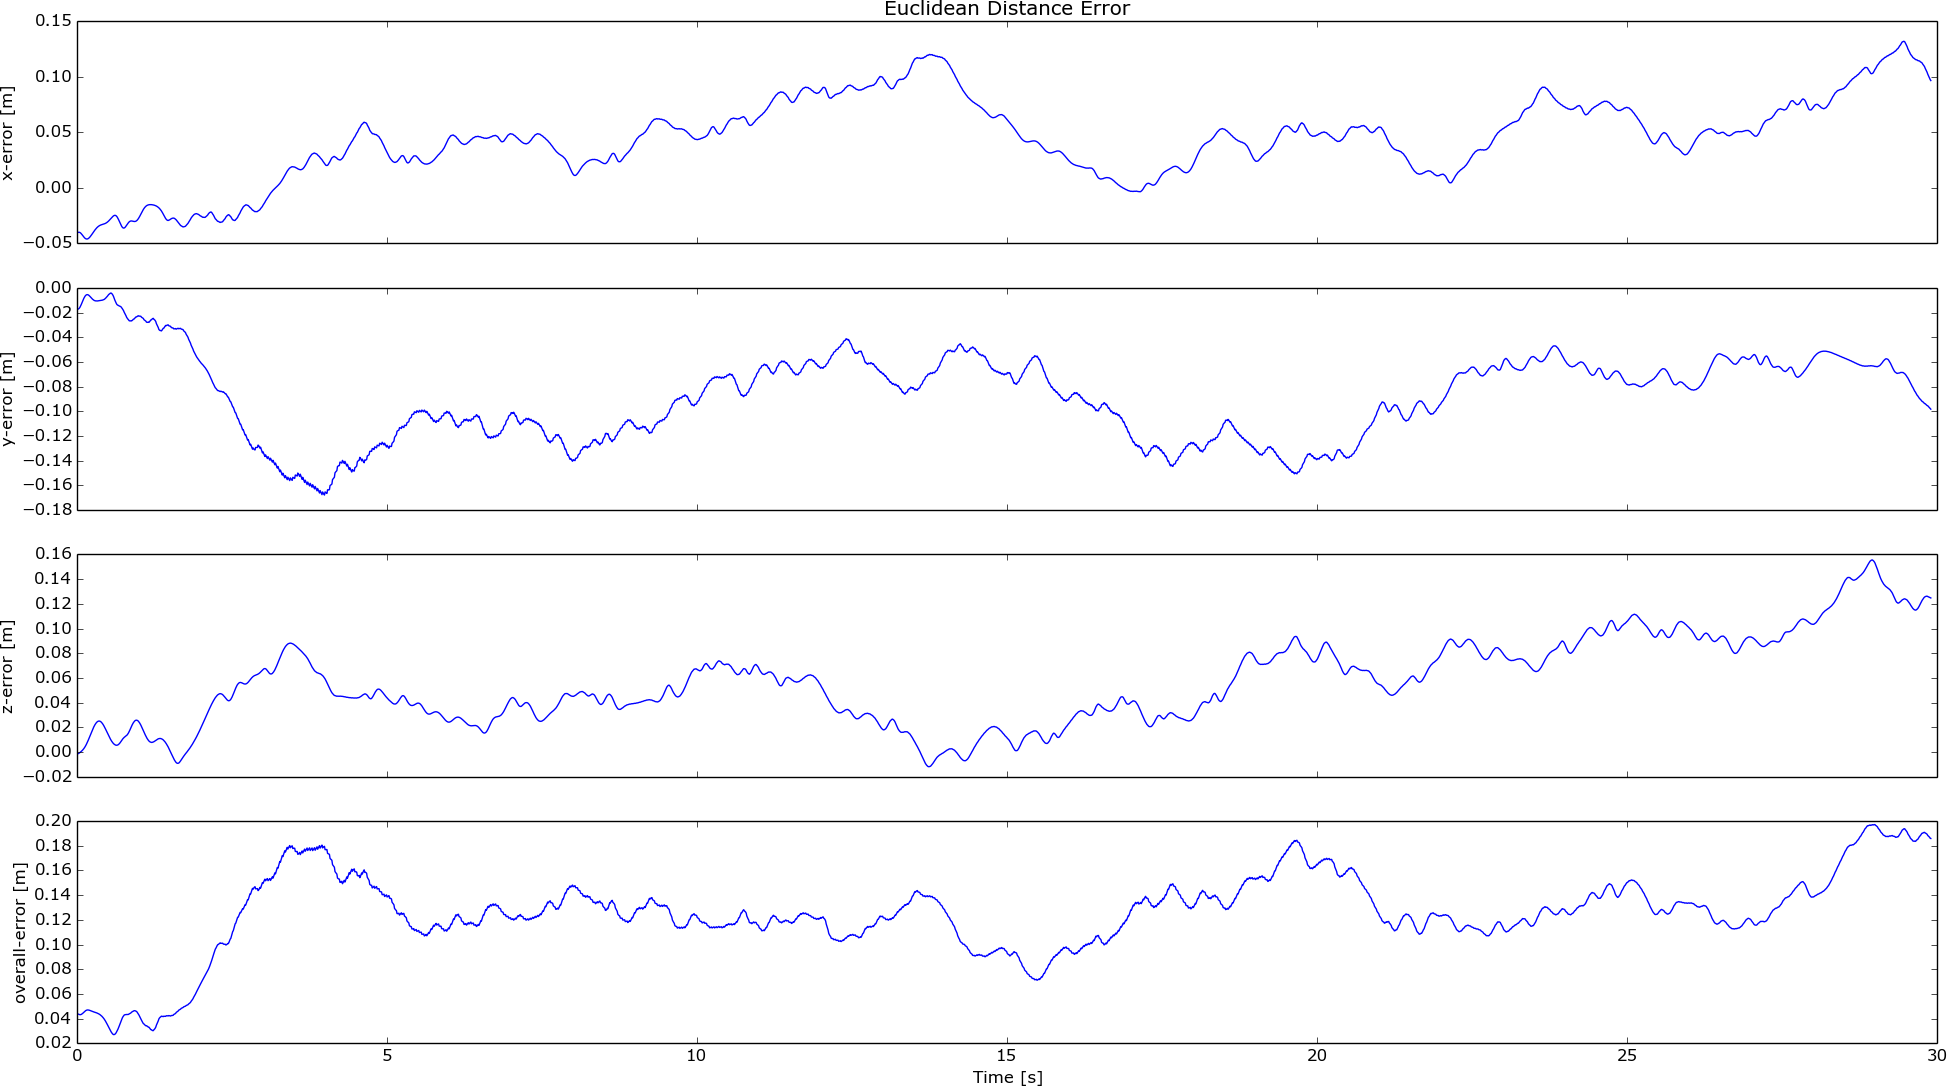
\includegraphics[width=0.45\textwidth]{CONTENT/Figure/figure5_2_a.png}
		\label{fig:fig5-2-a}}
	\end{subfloat}\qquad
	\begin{subfloat}[]{
		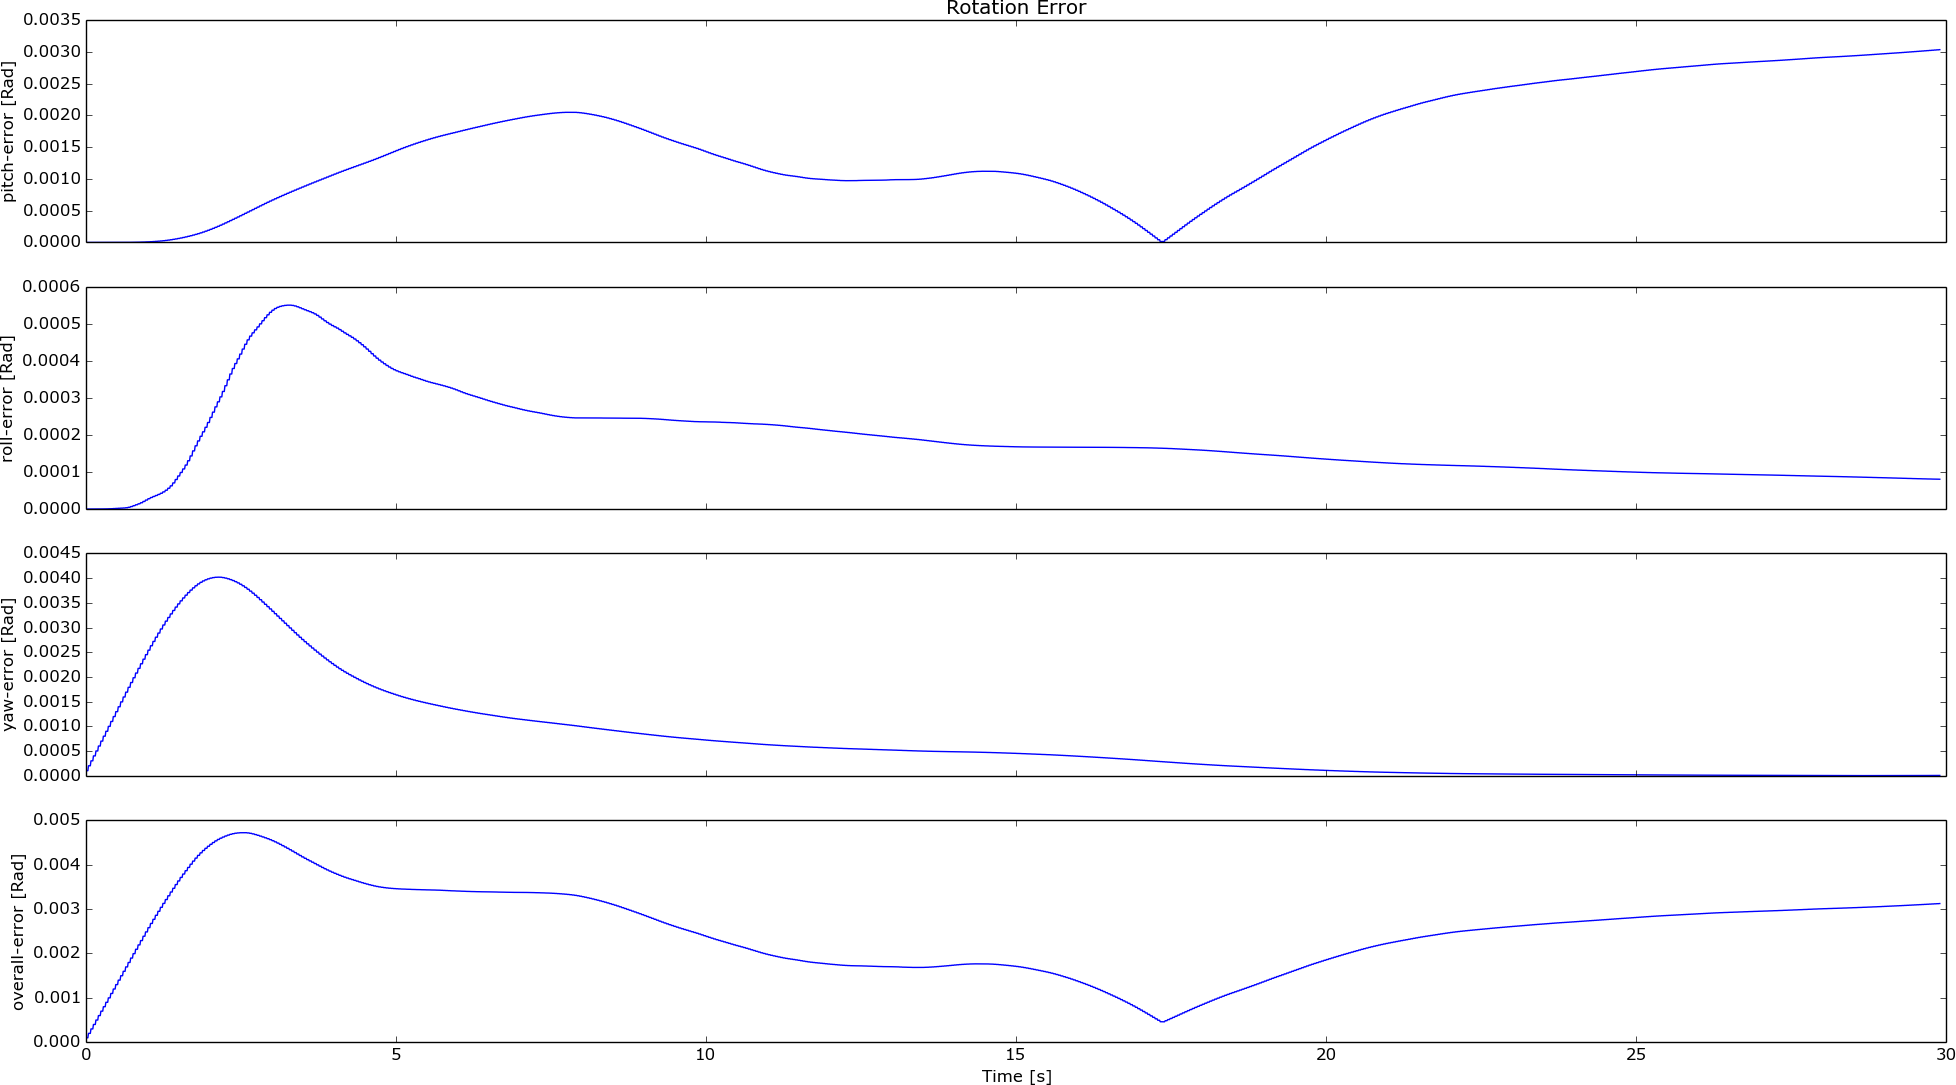
\includegraphics[width=0.45\textwidth]{CONTENT/Figure/figure5_2_b.png}
		\label{fig:fig5-2-b}}
	\end{subfloat}
		\begin{subfloat}[]{
		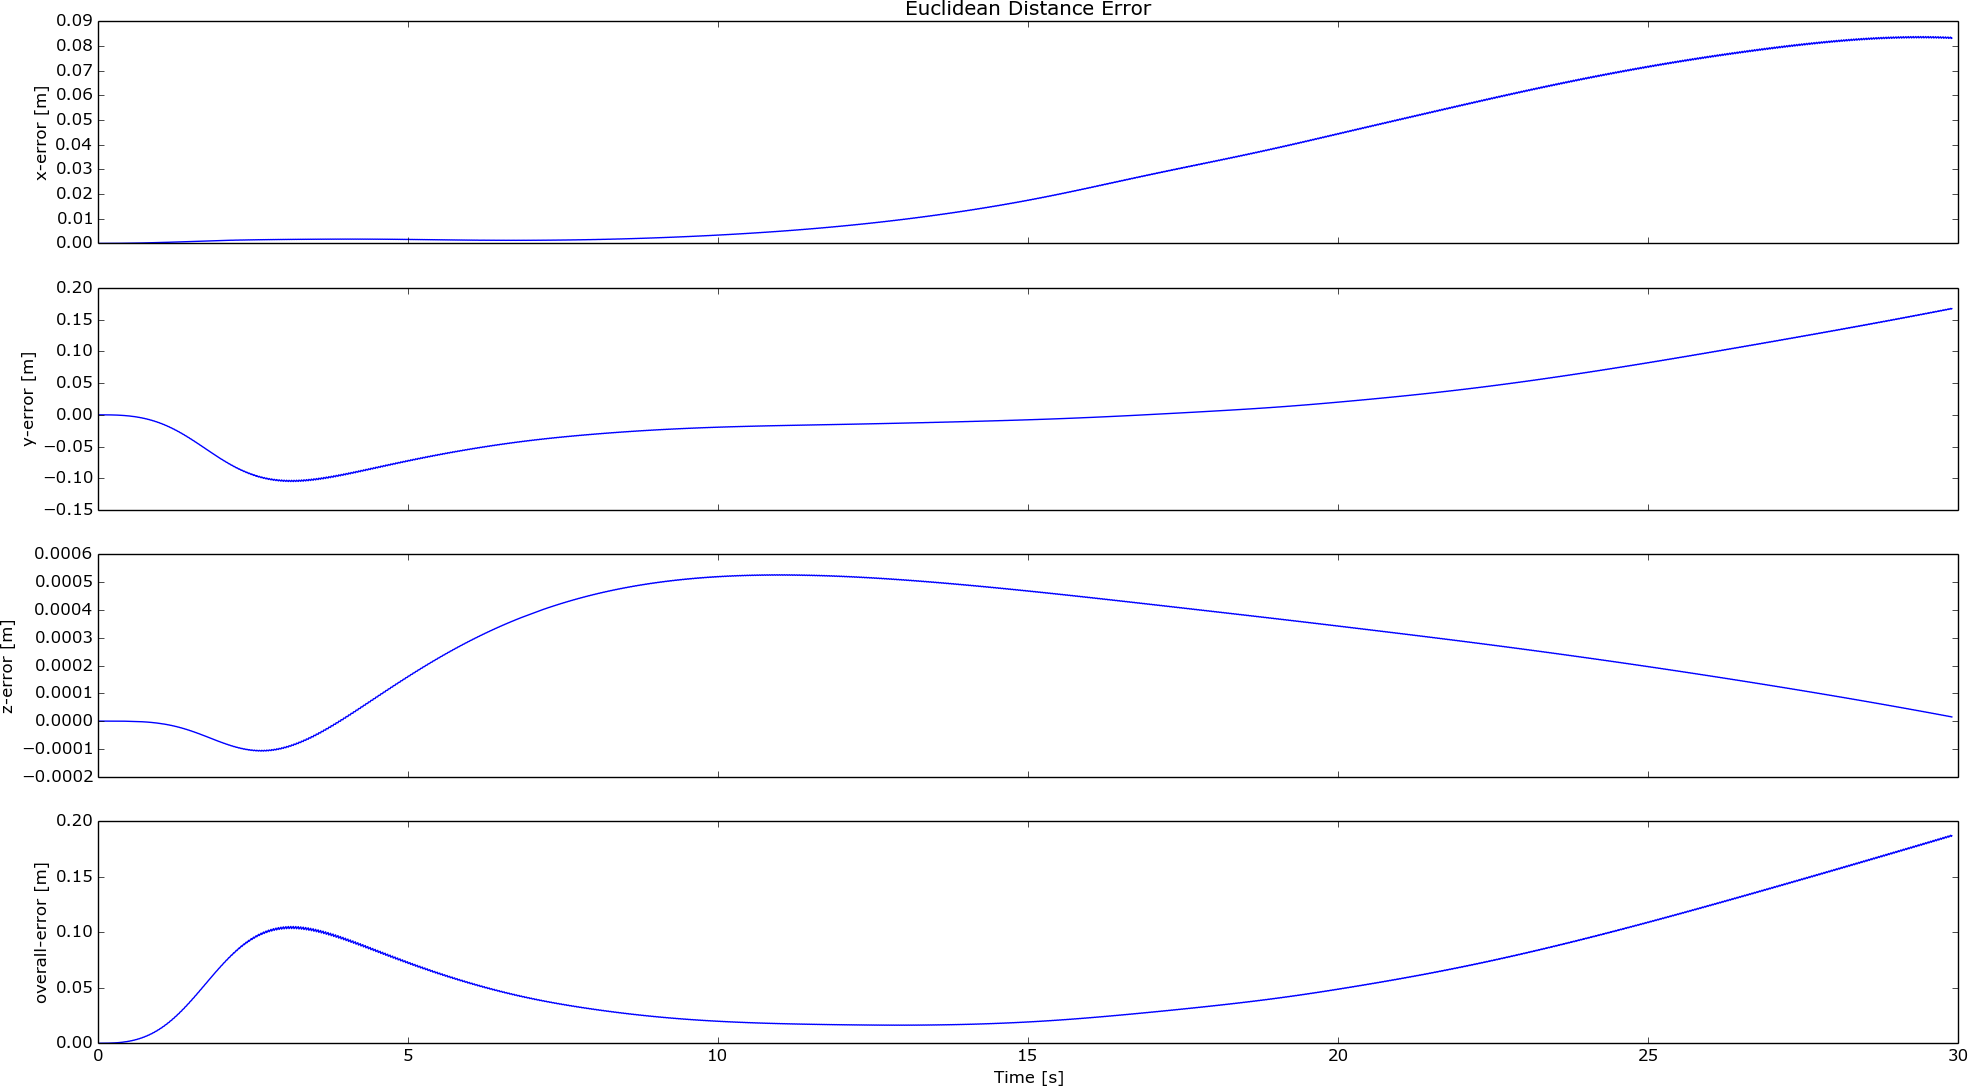
\includegraphics[width=0.45\textwidth]{CONTENT/Figure/figure5_2_c.png}
		\label{fig:fig5-2-c}}
	\end{subfloat}\qquad
	\begin{subfloat}[]{
		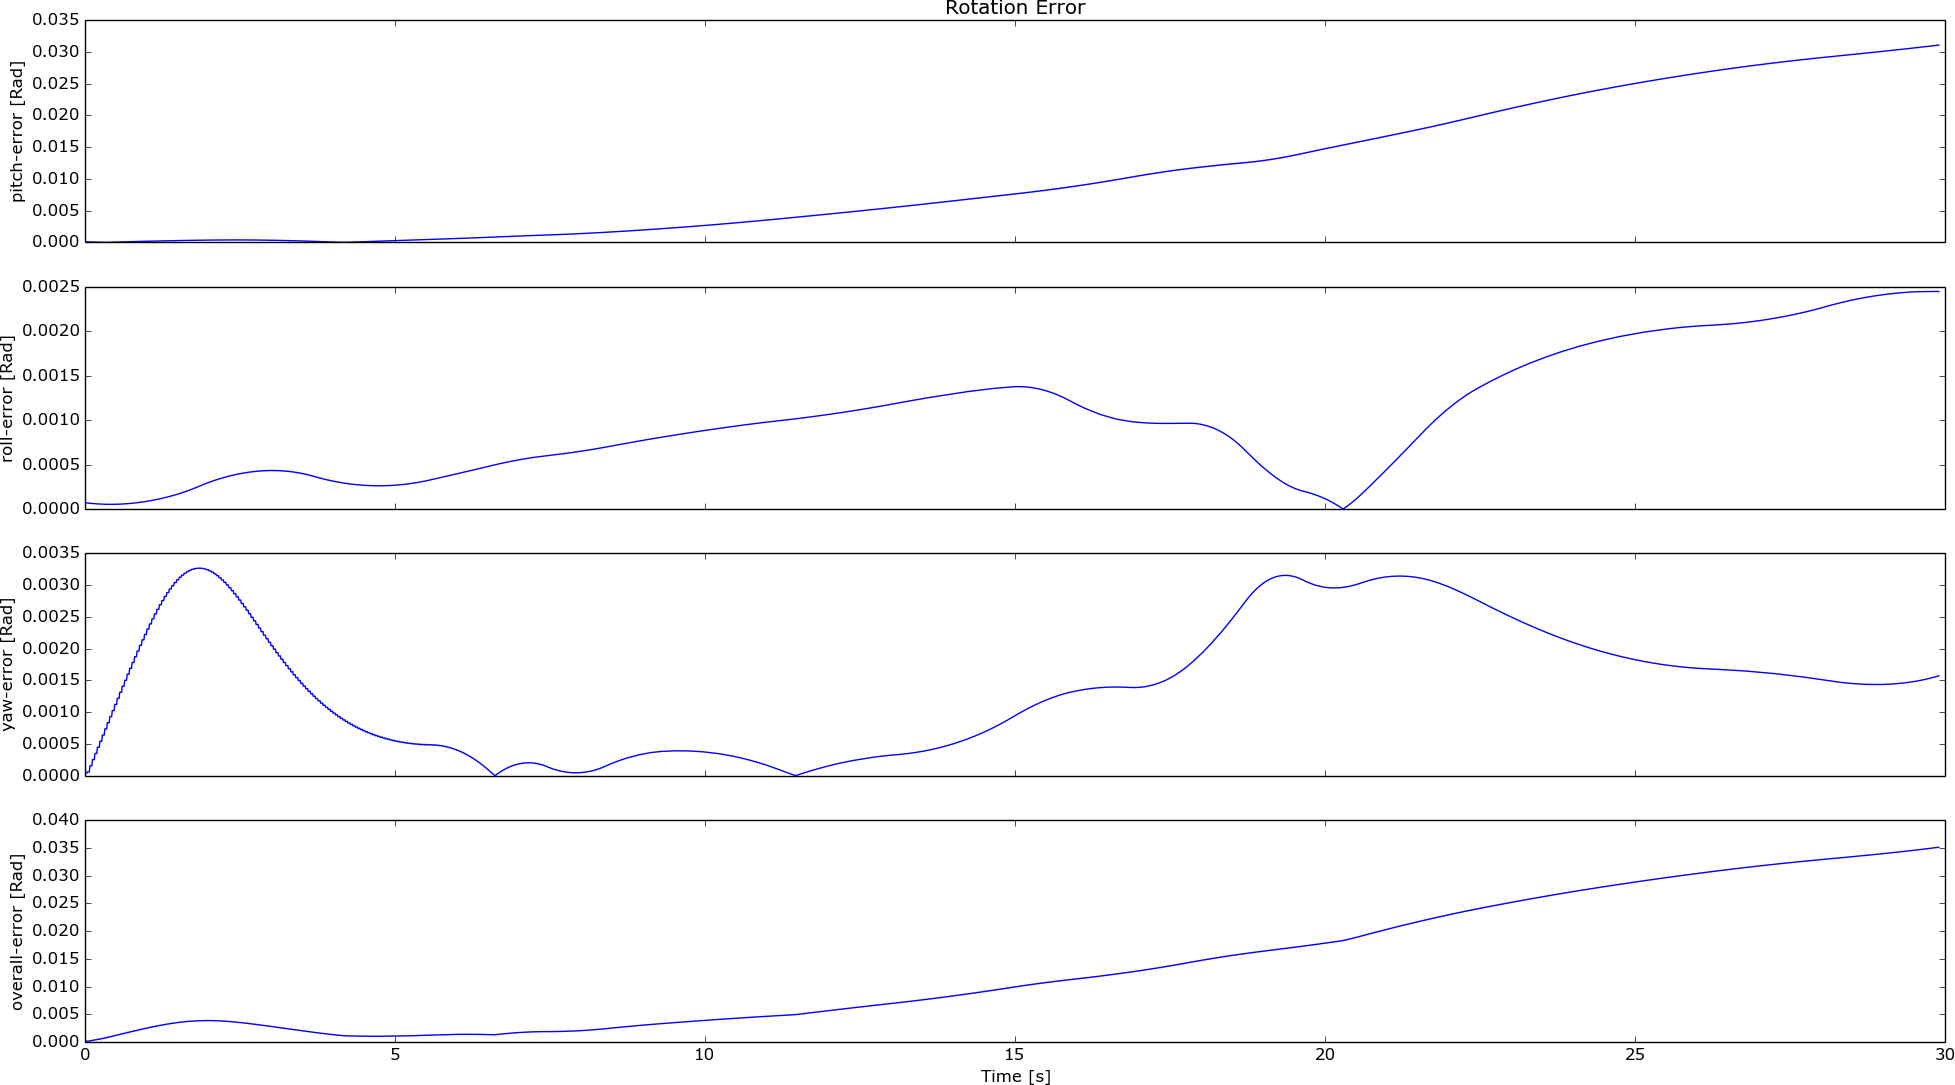
\includegraphics[width=0.45\textwidth]{CONTENT/Figure/figure5_2_d.png}
		\label{fig:fig5-2-d}}
	\end{subfloat}
		\begin{subfloat}[]{
		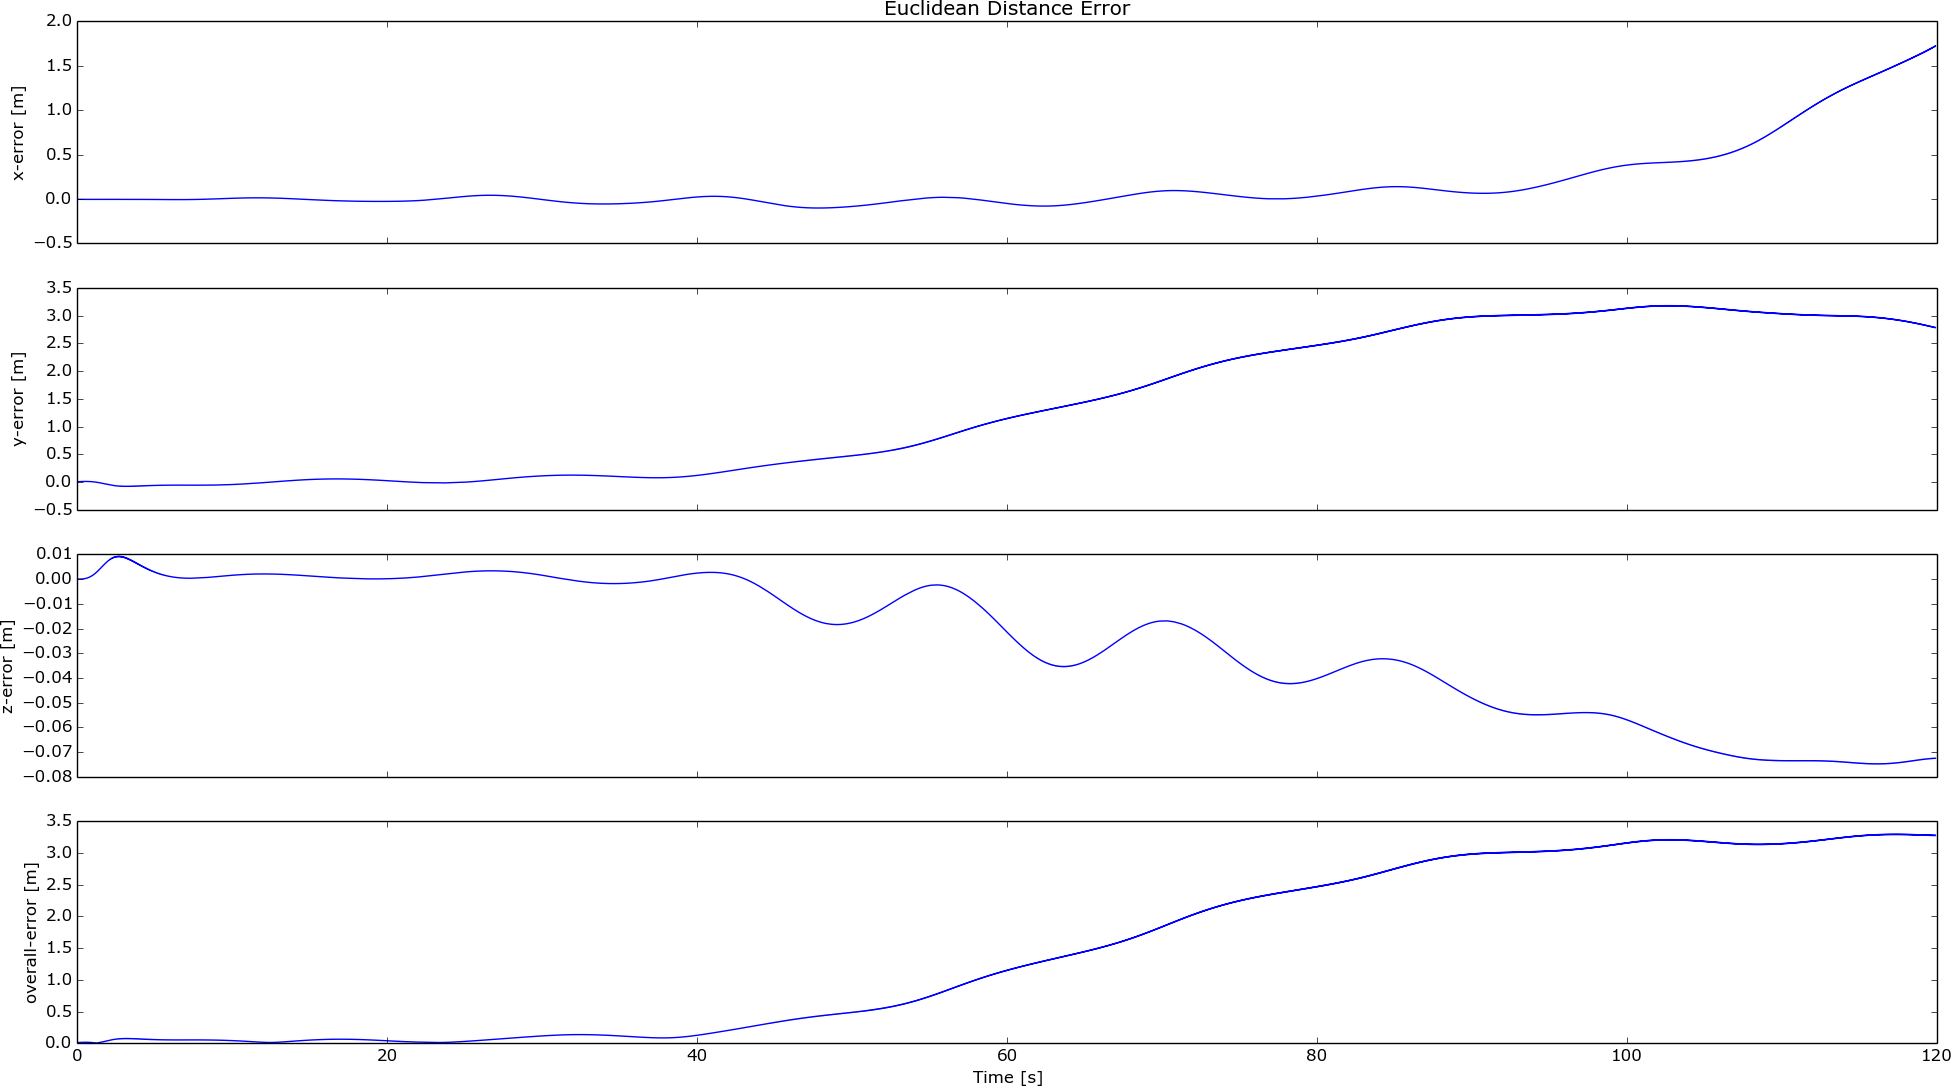
\includegraphics[width=0.45\textwidth]{CONTENT/Figure/figure5_2_e.png}
		\label{fig:fig5-2-e}}
	\end{subfloat}\qquad
	\begin{subfloat}[]{
		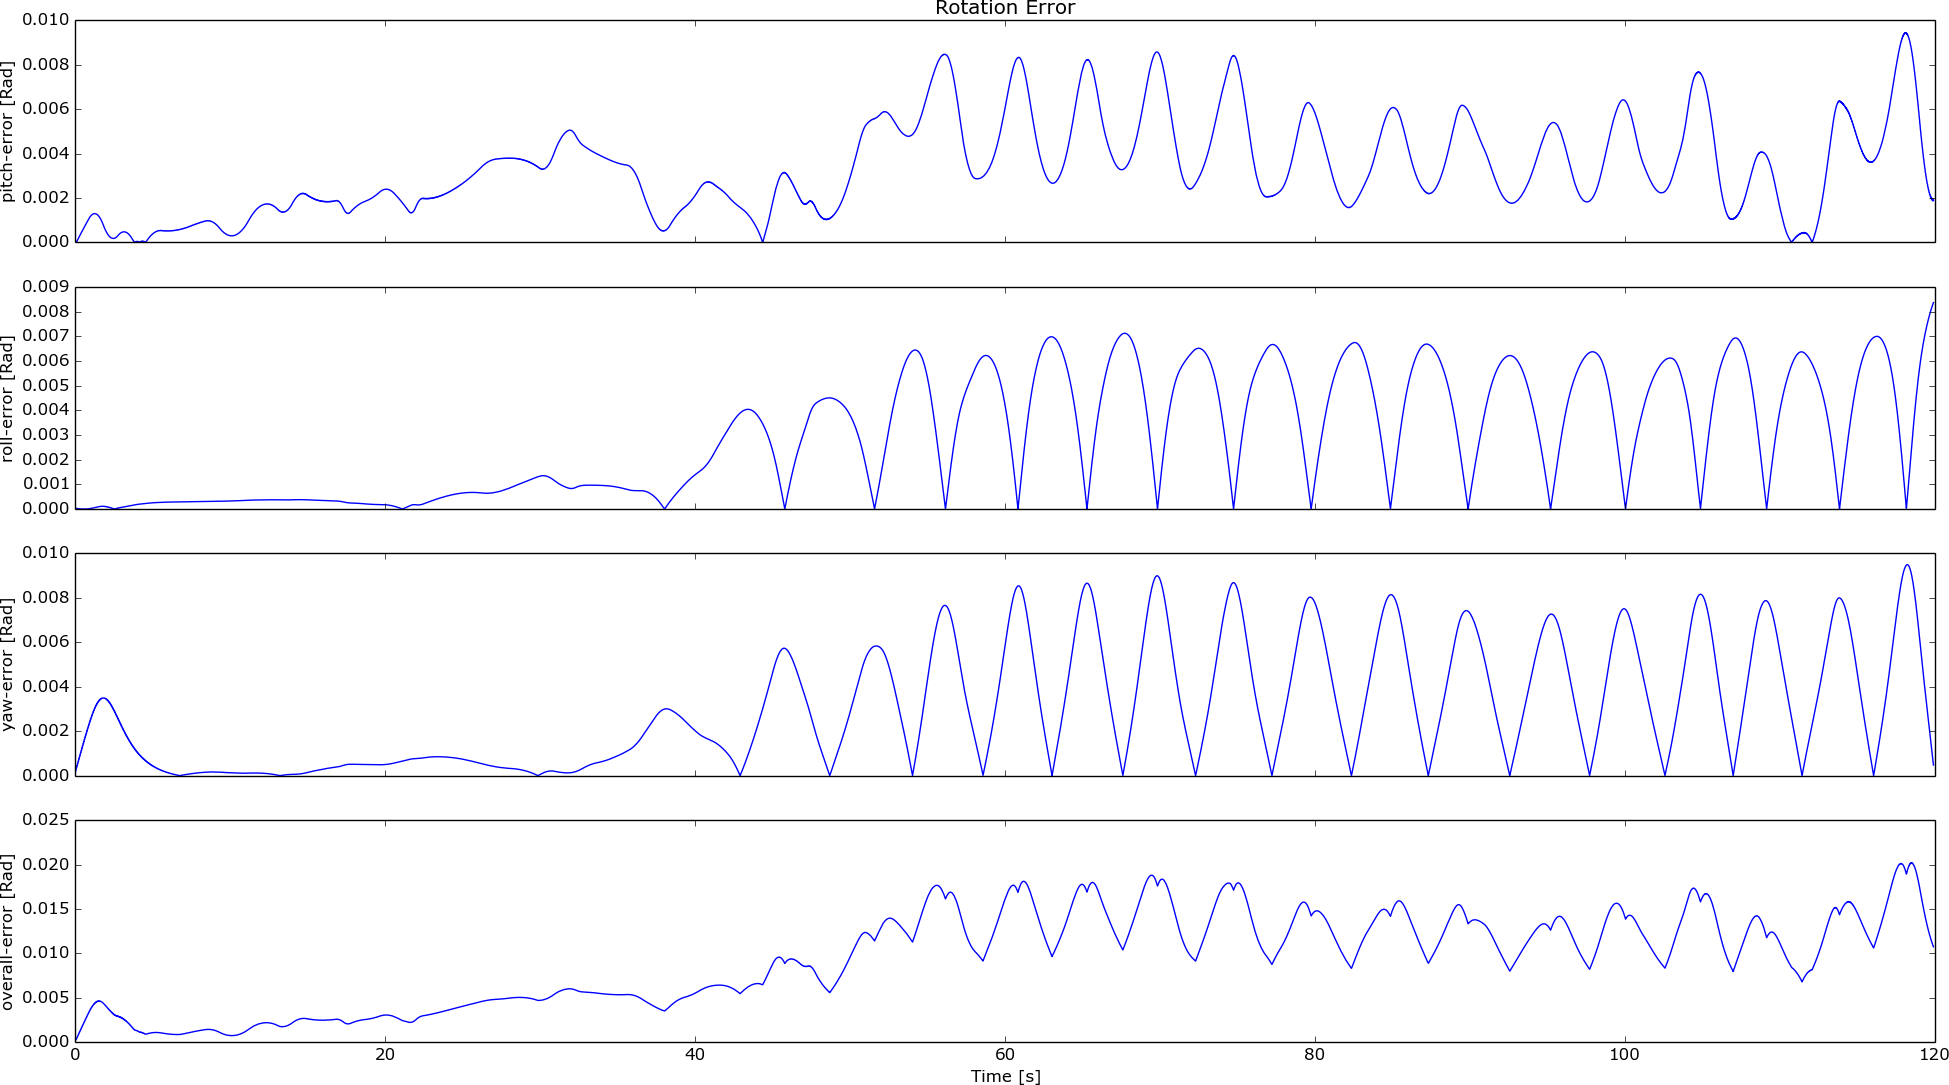
\includegraphics[width=0.45\textwidth]{CONTENT/Figure/figure5_2_f.png}
		\label{fig:fig5-2-f}}
	\end{subfloat}
	
	%\hspace*{\fill} % separation between the subfigures
	
	\caption{Experiment 1: (a)(b) Position and attitude drift of Dataset \textbf{001} (c)(d) Position and attitude drift of Dataset \textbf{002} (e)(f) Position and attitude drift of Dataset \textbf{004}. Position error is measured using Euclidean distance, and attitude drift is measured by transforming quaternion into Euler angle (see Appendix \ref{chap:appendix3}). Ground truth data is provided by synthetic IMU data generator.} 
	\label{fig:fig5-2}
\end{figure}

\begin{table}[t]
\centering
\begin{tabular}{|c || P{3cm} | P{3cm} | P{3cm} |} 
\hline
 Dataset & APD [m] & AAD [Rad] & TPD [ms] \\
 \hline
 001 & 0.1251 & 0.0025 & 0.0184 \\ 
 002 & 0.0622 & 0.0134 & 0.0188 \\ 
 004 & 1.4319 & 0.0094 & 0.0187 \\ 
 \hline
\end{tabular}
     \caption{Experiment 1: APD (Average Position Drift) and AAD (Average Attitude Drift) is measured by averaging overall position and attitude drift. For TPD (Time-elapsed Per Data), we run the experiment 100 times to measure a overall elapsed time, then divide by number of experiments and number of IMU measurements to obtain the single data processing time.}
    \label{table:tb3}
\end{table}

\subsection{Experiment 2: VIO Versus VO}
\label{subsec:experiment2}

In this experiment, we will compare our suggested VIO with single VO using same dataset sequences. As we have discussed before, correction data by visual sensor has a large impact on our final pose estimation since global translation and angle rotated around gravity vector (yaw) are unobservable for IMU, ESKF somehow needs those results if it is not aware of exact movement model. Here we run experiments roughly under the pipeline in Section \ref{sec:pipeline_summary} except we exclude the keyframe BA procedure, which we will discuss in next experiment.

The results of experiment 2 on trajectory \textbf{004} have been shown in Figure \ref{fig:fig5-3}. One can see from figure that VIO has lower variance than VO in translation though they have similar drift. VIO is better than VO in attitude drift since VIO gains much lower error than VO in two observable parameters (pitch and roll), we can also see that VIO and VO report the similar error trends in yaw. Overall such results are competitive among similar systems \cite{mourikis2007multi, forster2015imu}. We also evaluate the processing time using similar way as in Section \ref{subsec:experiment1}, VIO finally has an average time per IMU data as 4.570 [ms], which still runs in real-time.

We conclude that the performance of VO has a large impact on 3-vector global translation and rotational angle around gravity vector. However ESKF frame has lower variance and less drift in pitch and roll.

\begin{figure}
\centering
	\begin{subfloat}[]{
		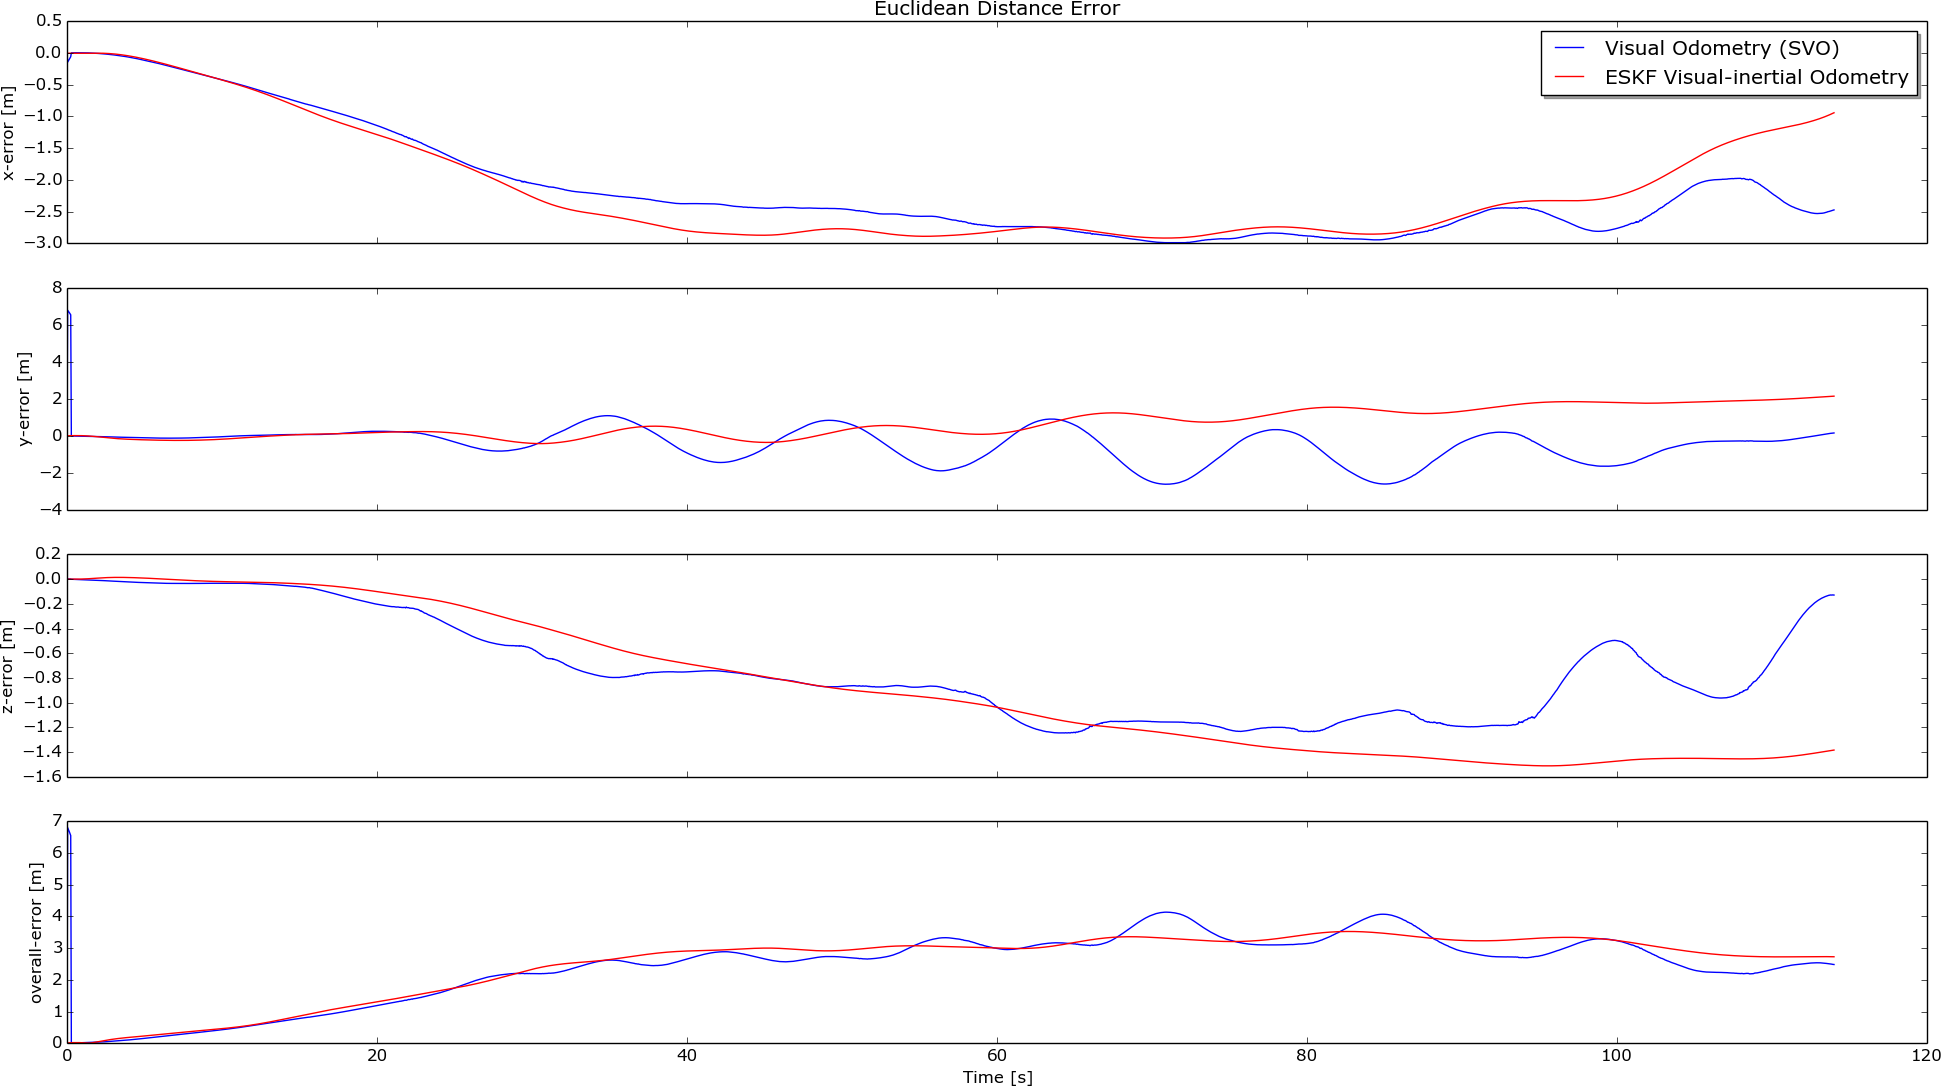
\includegraphics[width=0.45\textwidth]{CONTENT/Figure/figure5_3_a.png}
		\label{fig:fig5-3-a}}
	\end{subfloat}\qquad
	\begin{subfloat}[]{
		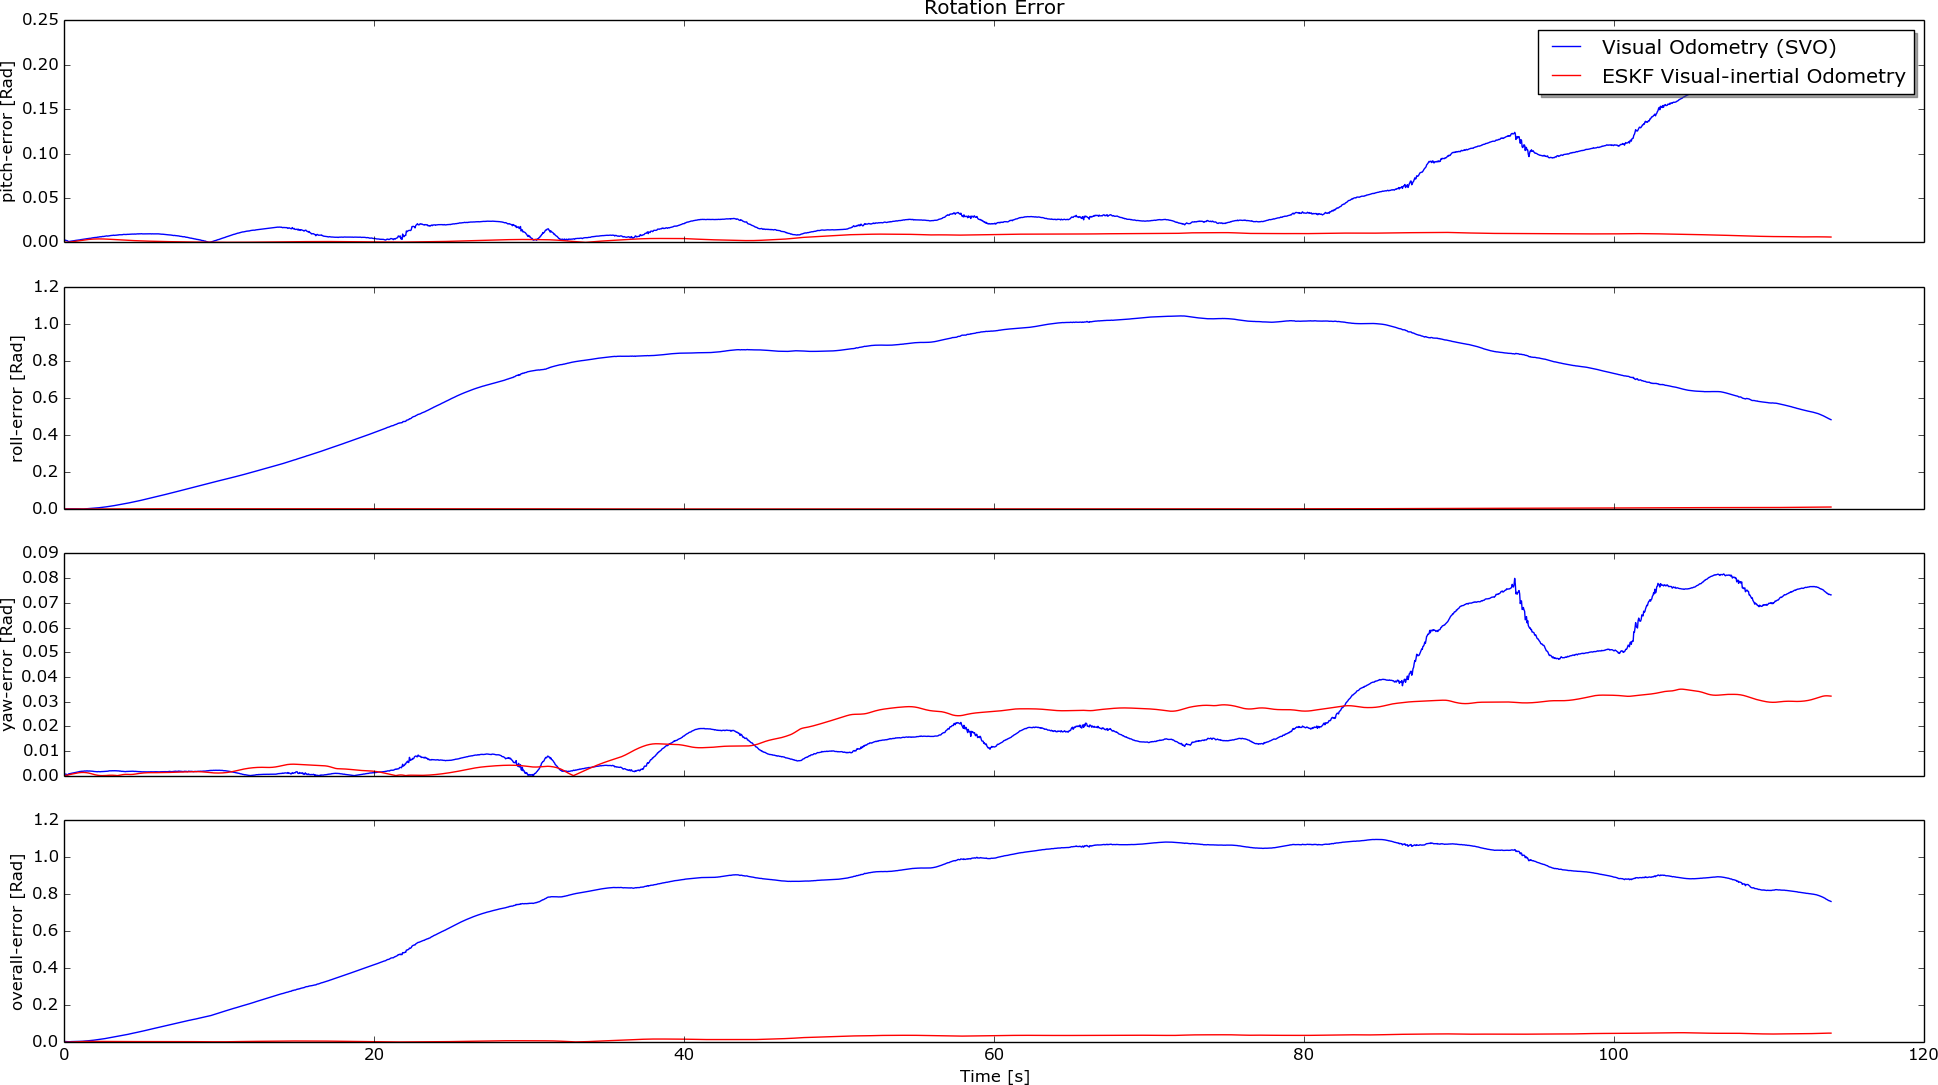
\includegraphics[width=0.45\textwidth]{CONTENT/Figure/figure5_3_b.png}
		\label{fig:fig5-3-b}}
	\end{subfloat}
	
	%\hspace*{\fill} % separation between the subfigures
	
	\caption{Experiment 2: (a) Position drift of VIO and VO. (b) Attitude drift of VIO and VO. Both VIO and VO report an average position drift less than 1\% of overall travelled distance, however VIO performs better than VO in attitude drift as VIO has 0.027 [rad] and VO has 0.787 [rad] average attitde drift.} 
	\label{fig:fig5-3}
\end{figure}

\subsection{Experiment 3: Keyframe Bundle Adjustment}
\label{subsec:experiment3}

We further show keyframe BA improves the estimation quality by performing experiment 3. In experiment 3, we run our VIO on trajectory \textbf{004} with and without kerframe BA. Each BA step only happens when new keyframe is inserted, it stops when meeting the maximum iteration number (we set this number to 10) or a threshold value. After BA step, an extra correction step will be applied on error state via the results from keyframe BA.

In Figure \ref{fig:fig5-4}, we report the results of VIO with BA and without BA. One can see that red curve (VIO with keyframe BA) is more close to zero for most time, which shows that keyframe BA improves the camera pose estimation quality. Moreover blue curve reports an average position drift of 2.67 [m], where red curve reports 2.49 [m], which concludes that VIO with keyframe BA have 10 \% less position drift than VIO without BA on average. For attitude, VIO with keyframe BA also have less drift than VIO without keyframe BA, which former reports an average attitude drift of 0.028 [rad] and the other is 0.029 [rad]. For processing time, keyframe BA increases approximately 0.5 [ms] for single IMU measurement on average, which leads to 5.08 [ms] per IMU measurement. 

We conclude that keyframe BA as a motion optimization step improves the estimation quality in our case, and within 10 maximum iteration for single BA solution turn, the whole system still runs in real-time.

\begin{figure}
\centering
	\begin{subfloat}[]{
		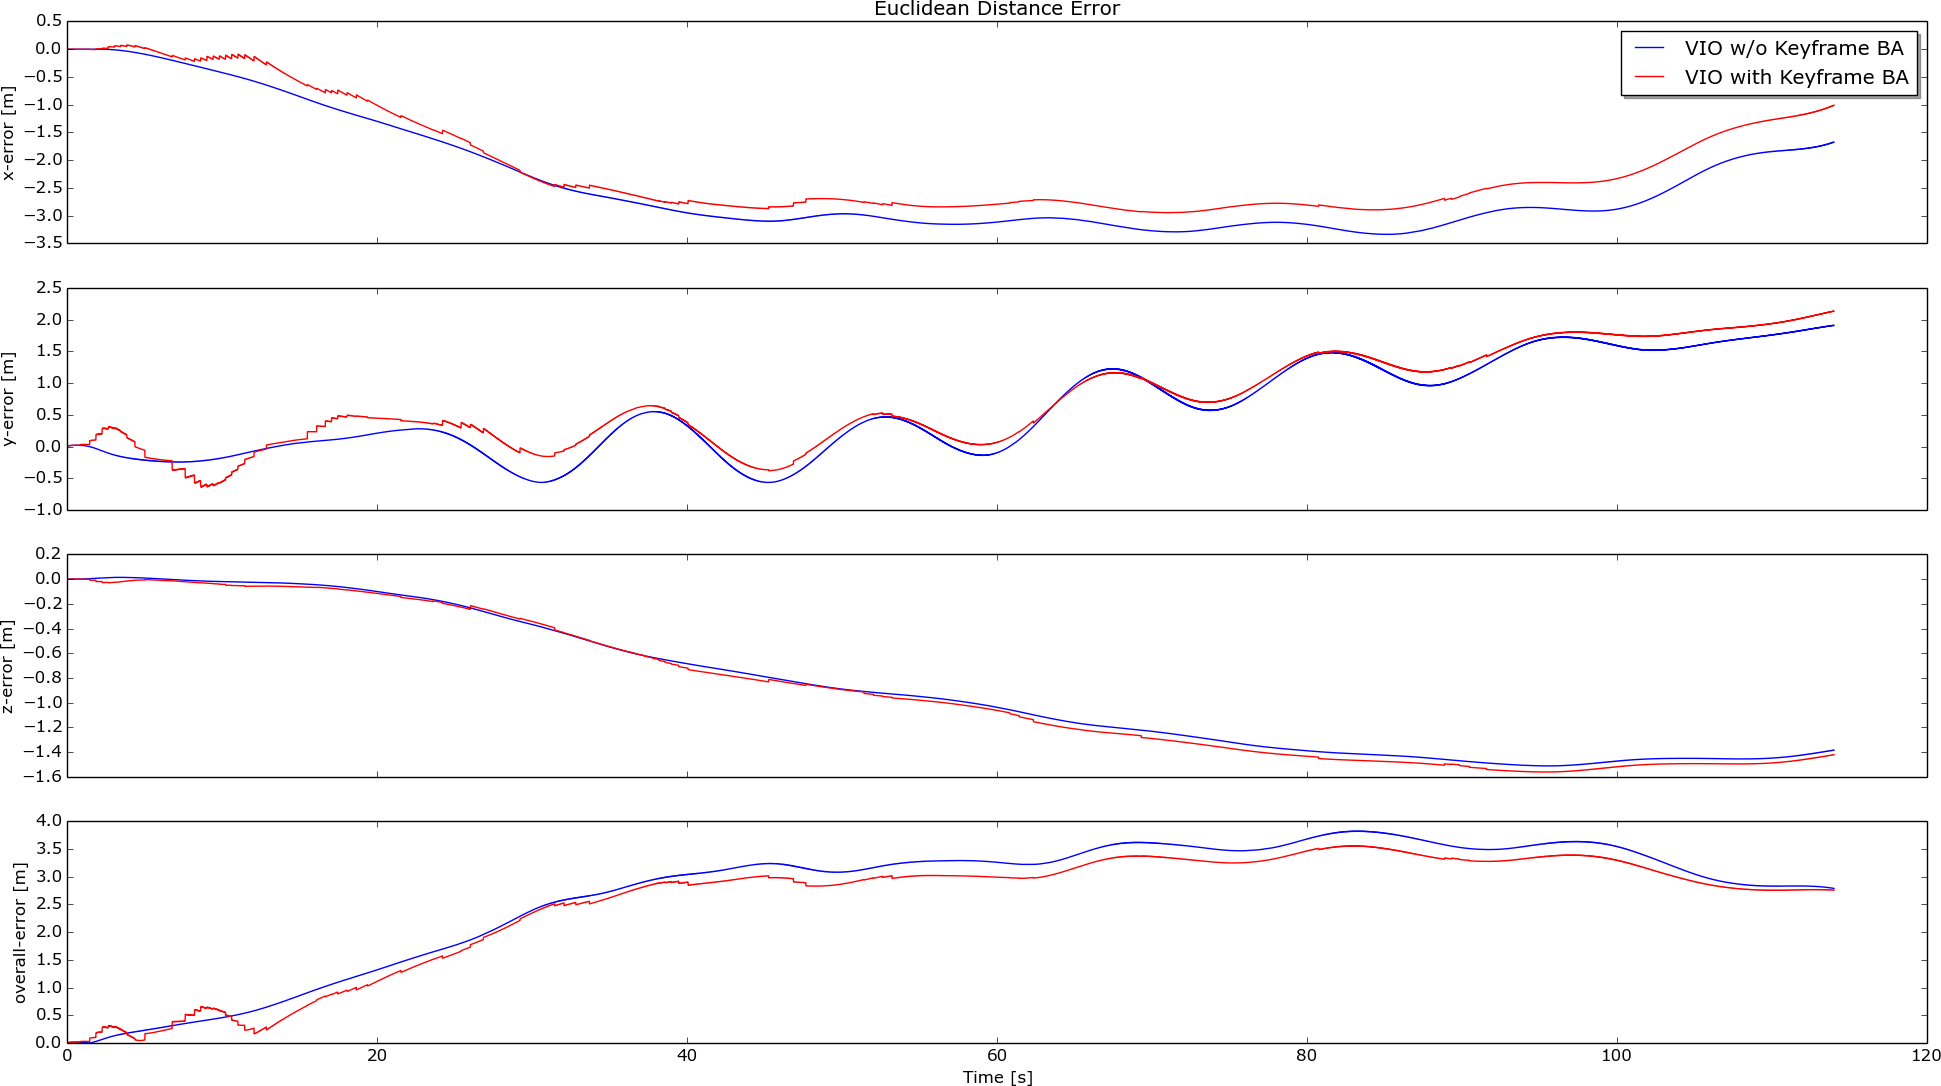
\includegraphics[width=0.45\textwidth]{CONTENT/Figure/figure5_4_a.png}
		\label{fig:fig5-4-a}}
	\end{subfloat}\qquad
	\begin{subfloat}[]{
		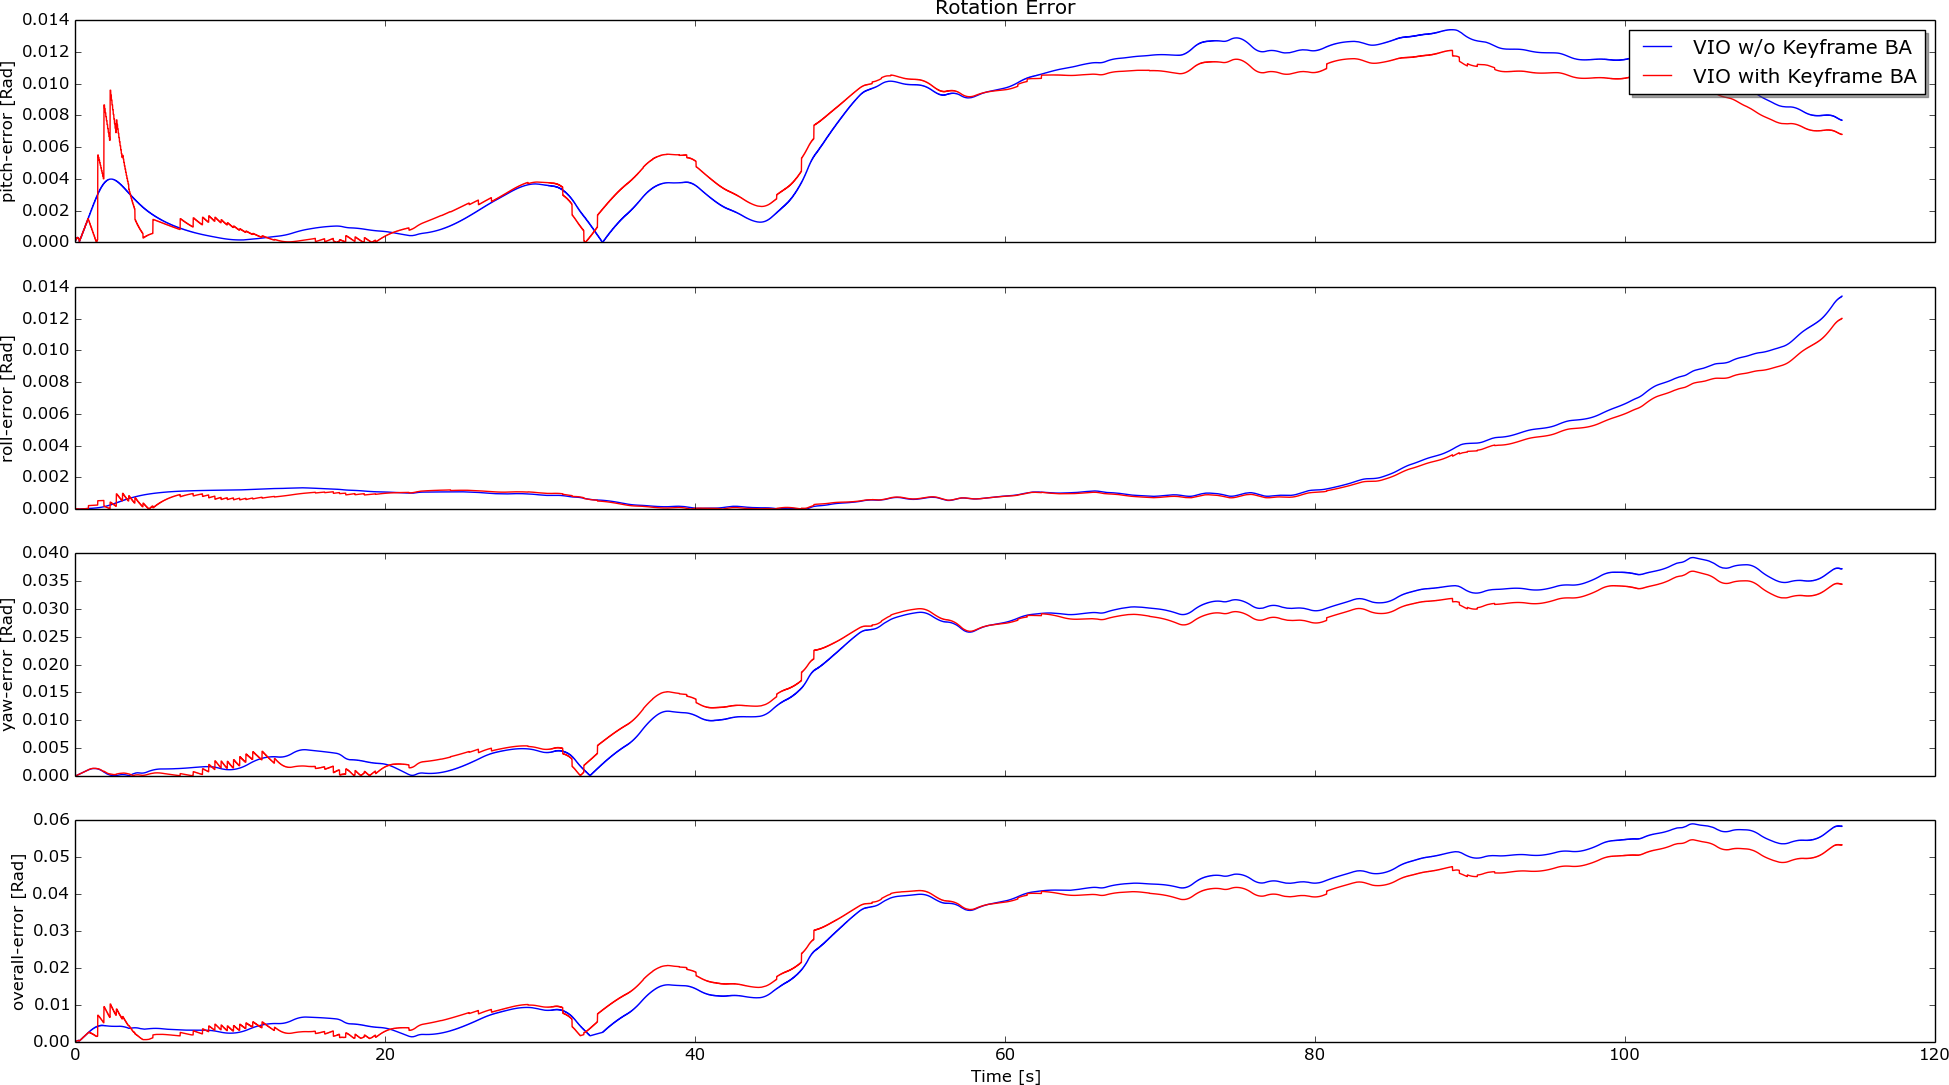
\includegraphics[width=0.45\textwidth]{CONTENT/Figure/figure5_4_b.png}
		\label{fig:fig5-4-b}}
	\end{subfloat}
	
	%\hspace*{\fill} % separation between the subfigures
	
	\caption{Experiment 3: (a) Position drift of VIO with and without BA. (b) Attitude drift of VIO with and without BA. The curve shows the error between estimation and ground truth, more close to zero is better.} 
	\label{fig:fig5-4}
\end{figure}

\subsection{Experiment 4: Runtime Evaluation}
\label{subsec:experiment4}


\begin{table}[t]
\centering
\begin{tabular}{|c | P{4cm} |} 
\hline
\ & Time Consuming [ms] \\
\hline
ESKF Prediction & 0.0146\\
Visual Odometry & 4.4656\\
ESKF Correction & 0.0422\\
Keyframe BA & 0.2671\\
\hline
\textbf{Total Visual-Inertial Odometry} & 4.7913\\
\hline

\end{tabular}
     \caption{Experiment 4: Break-up timing results.}
    \label{table:tb5}
\end{table}

\begin{table}[t]
\centering
\begin{tabular}{|c | P{7cm} | P{3cm} | } 
\hline
Name & Parameter Name & Value \\
\hline
\multirow{2}{*}{ESKF IMU} & Nominal state integration & Euler \\
				& Error state integration & Truncated Euler \\
\hline
\multirow{2}{*}{VO} & Max number of features per image & 120 \\
				& Max number of keyframes & 20 \\
\hline
\multirow{2}{*}{Keyframe BA} & Max number of camera poses & 20 \\
				& Max number of iterations & 10 \\
\hline
\end{tabular}
     \caption{Experiment 4: parameter settings in experiment 4, which follows settings as we explained in experiment 1, experiment 2 and experiment 3.}
    \label{table:tb4}
\end{table}

Table \ref{table:tb5} shows a break-up of average time consumption per IMU measurement to estimate camera motion in our synthetic datasets. In this experiment, we follow the parameter setting in former experiments, which explicitly shows in Table \ref{table:tb4}. We run experiments on Dataset \textbf{003} and Dataset \textbf{004} 100 times respectively to obtain the average processing time.

Though we have shown that our ESKF framework runs in constant time complexity, the whole VIO spends most of time on VO part. For VO part, we use \textit{Fast} parameter setting as \cite{forster2014svo} suggests except we compromise the maximum keyframe number to 20 to obtain a more accurate estimation results. The whole system runs smoothly in real-time with our virtual IMU sensor and camera settings, which needs 4.7913 [ms] to process single IMU measurement. The potential time left could be used to build and optimize a environmental map.

We conclude that the VIO we suggest in this master thesis have the ability to accomplish a real-time navigation task. It will further be significantly speed-up when more efficient and robust VO has been exploited.


\section{Conclusion}
\label{sec:exp_conclusion}

We first explain the reasons and ways we generate synthetic datasets in this chapter. Then we demonstrate four experiments on our synthetic dataset. In experiment 1, we use ground truth data in correction step, showing that if the extrasensory data gives us a good camera pose estimation, our visual-inertial odometry will obtain very little position drift (less than 0.55\% of overall distance travelled) and attitude drift (average 0.0134 [rad]); In experiment 2, we compare our visual-inertial odometry with state-of-art visual odometry SVO, the final results show that our method have less variation in position drift and huge improvement (0.027 [rad] vs 0.787 [rad]) in average attitude drift with regarding to SVO; In experiment 3, we further show that keyframe BA we propose decrease the overall position drift and attitude drift; We examine the time consumption in experiment 4, which shows our odometry runs in real-time with our virtual IMU (~100 HZ) and camera (~25 Hz).

Due to the time limits, we are not available to perform more experiments, \eg, using different visual odometry or on more realistic dataset. However the results we obtain in above experiments have shown that the keyframe-based visual-inertial odometry we suggest is robust, efficient and high accuracy. 